\documentclass[a4paper,12pt]{article}
\usepackage[utf8]{inputenc}  % Soporte para caracteres UTF-8
\usepackage{amsmath, amssymb} % Paquetes para matemáticas
\usepackage{graphicx} % Para incluir imágenes
\usepackage{hyperref} % Para enlaces y referencias cruzadas
\usepackage{booktabs}
\usepackage{geometry}
\usepackage{authblk}
\usepackage{float} 
\usepackage{array}
\usepackage{geometry} % Para ajustar márgenes
\geometry{margin=1in} % Márgenes de 1 pulgada

\begin{document}
\title{Comparison of Time Series Models of Solar Photovoltaic Electricity Generation in North of Mexico City}
\author{Ponciano J. Escamilla-Ambrosio\textsuperscript{1}[0000-1111-2222-3333]}
\author{Ricardo Alcaraz-Fraga\textsuperscript{2}}
\author{Gilberto L. Martinez-Luna\textsuperscript{1}[0000-0002-0105-1112]}

\affil{\textsuperscript{1}Instituto Politécnico Nacional, Centro de Investigación en Computación, Ciudad de México 07700, Mexico}
\affil{\textsuperscript{2}Instituto Politécnico Nacional, Escuela Superior de Física y Matemáticas, Ciudad de México 07700, Mexico}

\maketitle

\begin{abstract}
This paper presents a comprehensive comparison between classical time series prediction models, such as ARIMA, and more advanced approaches based on neural networks, specifically Long Short-Term Memory (LSTM) applied to solar generation data. Multiple datasets from different domains are evaluated with the aim of determining which model offers better performance in terms of accuracy and generalization ability. The results show that, while traditional models offer interpretability and are effective in certain situations, LSTM-based models outperform them in complex problems with long-term dependencies. Furthermore, the advantages and disadvantages of each approach are discussed based on computational requirements and the amount of data needed for effective training. This study provides a practical guide for selecting the appropriate model depending on the context and the available data.
\end{abstract}

\section{Introduction}
Solar photovoltaic (SPV) power generation is inherently dependent on various environmental factors, such as sunlight intensity, temperature, and weather conditions, which can vary significantly over time. Accurate forecasting of SPV energy output is essential for integrating this renewable energy source into existing power grids and ensuring its stability and reliability. Traditional time series models, such as ARIMA and Holt-Winters, have been widely used for forecasting in various domains due to their simplicity and interpretability. However, these models often struggle to capture complex, nonlinear patterns present in renewable energy data, especially when dealing with long-term dependencies.

In recent years, more advanced methods based on neural networks, particularly Long Short-Term Memory (LSTM) networks, have gained attention for their ability to model sequential data with intricate patterns. LSTM networks, a type of recurrent neural network (RNN), are specifically designed to handle long-term dependencies, making them suitable for time series prediction tasks with variable dynamics and nonlinearity.

This study aims to compare the performance of traditional time series models and LSTM networks in forecasting SPV energy output. By evaluating these models on real-world datasets, we seek to identify the advantages and limitations of each approach, providing insights into their applicability for energy forecasting in renewable energy systems.

\section{Related Work}
Nowadays green power generation, such as SPV is becoming of great interest. Never-
theless, there are some points to be considered when it comes to generate energy by this
means and get connected to the grid. One problem is that solar photovoltaic generation
is not constant; therefore, there is the need for a reliable photovoltaic power prediction,
where clustering analysis is a first step. The authors in [1] propose a clustering analysis,
which enhances the accuracy of the prediction model of RBF (Radial Basis Function)
photovoltaic power. The method is divided into time series analysis method, artificial
neural networks, support vector machine, etc. Then, meteorological information is fed
to the RBF and the back propagation (BP) neural network in order to predict the pho-
tovoltaic power generation. Although the method is quite accurate there are still some
issues that need to be considered, for example, improve data processing, strengthening
clusters analysis and enhancing extraction modes.  

In [2] the authors search and propose a new methodology to classify data of off grid
solar energy. They analyzed the curves of the voltage and current obtained from a pho-
tovoltaic station formed of 24 solar panels for three years in order to understand the
behavior of the energy obtained. They classified 5 types of situations which led to a
better understanding of the solar station to develop robust prediction algorithms. For
the study the authors divided the day into two, daytime taken as charge, and the dis-
charge when there were no generation or sunlight. And instead of processing the whole
curves that were produced during the day they took seven curves characeristics to train the algorithm. For pattern recognition, cluster search and database visualization,
SOM (Self Organized Maps) was used.  

Prediction of solar radiation is quite important for photovoltaic power generation. In
[3] the authors propose the use of neural networks to model such prediction. The ro-
bustness of the neural network depends on the type of data obtained from the photovol-
taic network study. Then, the type of data used to train the neural network is important
as well as the way this data is processed. Pre-processing and dividing the data gives a
better approximation model. To pre-process the data usually clustering is used for train-
ing a neural network. In their work, the authors proposed a prediction model for soiled
photovoltaic modules, as it was observed that dust on the panels may lead to power loss of up to 30\%. They considered soil characteristics such as physical, chemical, or spec-
tral properties and used specialized data processing techniques to improve the accuracy
of prediction.  

Connecting photovoltaic power into the electrical grid requires an accurate analysis
and simulation as the power output fluctuation may have negative effects to the grid. In
the work presented in [4], the ideal number of clusters for photovoltaic power patterns
data is determined that would achieve the best results. Here, a combination of conven-
tional clustering algorithms and bio-inspired optimization clustering algorithms was
presented. Clustering of photovoltaic power patterns is realized by utilizing a pattern
recognition methodology on historical data such as irradiance and ambient temperature
for a couple of years.  

Trying to predict solar radiation for photovoltaic power generation brings about the
big problem that even small changes in weather conditions really affect radiation. That
is why modelling forecasting is so important and will help in the determination of the
best possible number of clusters. First, time forecasting is divided into different condi-
tions so modelling can be applied to specific environments, at this point two processes
are required: clustering and classification. Clustering (unsupervised process) consists
in characterize and label the types of each time period in the training data. Classification
(supervised process) identifies the category of a time period in the forecasting stage. In
[5] the authors propose an enhanced solar data clustering, pattern recognition and fore-
casting learning abilities simultaneously for an accurate weather forecasting. A cluster-
ing method is developed that only uses global horizontal radiance. After that, pattern
recognition identifies the cluster to which a forecasting day belongs with first few
hour\'s data. Finally, a two-layer machine learning based multimodel forecasting frame-
work is developed to strengthen learning abilities for the machine learning models.

\section{Solar Photovoltaic Electricity Generation Prediction}
In this section, the solar photovoltaic electricity generation plant installed at CIC-IPN
is described, along with the electricity generation data that have been obtained since the
activation of the SPV plant. Afterwards, time series forecasting of the collected data is performed and the results obtained are presented.

\subsection{Solar Photovoltaic Plant}
The data used were obtained from the solar photovoltaic (SPV) electricity generation
plant installed at CIC-IPN [6], located in north Mexico City, 19° 30' 11.1" North-lati-
tude, 99° 08' 52.1" West-longitude at 2,243 m altitude, see Fig.1. The SPV plant has
186 solar panels (Canadian Solar CS3U), connected to three inverters (each Fronius
Symo, 22.7 kW) with a maximum power capacity of 66.96 kW.

\subsection{SPV Data}
Data collected from this SPV plant includes several parameters, but the ones used in
this research include photovoltaic production (Wh), irradiance (W/m2), ambient tem-
perature (°C), panel temperature (°C) and variables related to the electric current of the sensors contained on the SPV panels (A). This data corresponds to 1101 days ranging from 25-10-2019 to 31-12-2023.

\section{Time Series Analysis}

Time series analysis involves examining data points collected or recorded at specific time intervals to identify patterns, trends, and relationships within the data. This type of analysis is crucial in various fields, including economics, finance, weather forecasting, and energy production, as it allows for modeling and predicting future outcomes based on historical data.

A fundamental aspect of time series analysis is understanding the components that constitute a time series[6]. These components typically include:

\begin{itemize}
    \item \textbf{Trend}: The long-term movement or direction in the data, indicating whether the series is increasing, decreasing, or remaining constant over time.
    \item \textbf{Seasonality}: Regular, periodic fluctuations that occur within the series, often corresponding to specific times of the year, month, or week.
    \item \textbf{Cyclic Patterns}: Non-seasonal, long-term oscillations that can be attributed to economic cycles, technological advancements, or other systemic factors.
    \item \textbf{Random Variation}: The irregular, unpredictable fluctuations that do not follow a pattern and are often considered as noise.
\end{itemize}

Identifying and analyzing these components help in building accurate models for forecasting and understanding the underlying processes generating the data. Techniques such as decomposition methods, autocorrelation analysis, and spectral analysis are commonly employed to dissect and interpret time series data.

In the context of this study, time series analysis is pivotal for understanding the temporal patterns in solar photovoltaic (SPV) energy production. By analyzing the time series data of SPV output, we can develop models to predict future energy generation, which is essential for efficient energy planning and grid integration.

\subsection{ARIMA}

The ARIMA (AutoRegressive Integrated Moving Average) model is one of the most widely used methodologies for time series analysis and forecasting. ARIMA combines three key components: the autoregressive (AR) model, the moving average (MA) model, and integration (I), which is used to transform a non-stationary series into a stationary one[7].

The AR component describes the dependence of the current values of the series on its past values. The MA component, on the other hand, models the dependence of current values on past errors. Finally, the integrated (I) part is used to difference the series, removing non-stationary trends.

A significant advantage of the ARIMA model is its ability to adapt to univariate time series that exhibit non-stationary behavior without requiring complex transformations. Moreover, ARIMA has become a standard tool across various fields, from finance to engineering, due to its simplicity and effectiveness in forecasting.

The ARIMA model can be mathematically expressed as ARIMA$(p,d,q)$, where $p$ is the order of the autoregressive component, $d$ is the number of differences applied to make the series stationary, and $q$ is the order of the moving average component. The general equation for an ARIMA model is as follows:

\[
y_t = c + \phi_1 y_{t-1} + \cdots + \phi_p y_{t-p} + \theta_1 \epsilon_{t-1} + \cdots + \theta_q \epsilon_{t-q} + \epsilon_t
\]

where $y_t$ is the value observed at time $t$, $c$ is a constant, $\phi_i$ are the coefficients of the AR component, $\theta_j$ are the coefficients of the MA component, and $\epsilon_t$ is a random error term.

\section{Deep Neural Networks}

Neural networks have emerged as a powerful class of models for solving complex problems in various domains, including computer vision, natural language processing, and time series forecasting. Inspired by the biological neural networks in the human brain, artificial neural networks (ANNs) consist of interconnected nodes, or neurons, that process information in a layered architecture[8].

A typical neural network can be mathematically represented as follows:

\begin{equation}
Y = f(W \cdot X + b)
\end{equation}

where:
\begin{itemize}
    \item \(Y\) is the output vector,
    \item \(f\) is the activation function (e.g., sigmoid, ReLU),
    \item \(W\) is the weight matrix,
    \item \(X\) is the input vector,
    \item \(b\) is the bias vector.
\end{itemize}

The activation function introduces non-linearity into the model, enabling it to learn complex patterns. Common choices for activation functions include:

\begin{itemize}
    \item Sigmoid: \(f(x) = \frac{1}{1 + e^{-x}}\)
    \item Hyperbolic Tangent: \(f(x) = \tanh(x)\)
    \item Rectified Linear Unit (ReLU): \(f(x) = \max(0, x)\)
\end{itemize}

The training process of a neural network involves optimizing the weights and biases to minimize the loss function, which quantifies the difference between the predicted outputs and the actual targets. A popular choice for the loss function in regression tasks is the mean squared error (MSE):

\begin{equation}
L = \frac{1}{n} \sum_{i=1}^{n} (y_i - \hat{y}_i)^2
\end{equation}

where \(y_i\) is the actual output and \(\hat{y}_i\) is the predicted output.

Recent advancements in deep learning, particularly with the introduction of deep neural networks (DNNs), have further enhanced the capability of neural networks to model high-dimensional data.

\subsection{LSTM}

Long Short-Term Memory (LSTM) networks are a specialized type of recurrent neural network (RNN) designed to effectively capture long-range dependencies in sequential data. Traditional RNNs suffer from issues such as vanishing and exploding gradients, which make it difficult for them to learn long-term patterns. LSTMs address this limitation through their unique architecture, enabling them to retain information over extended periods[9].

The LSTM unit consists of a cell state, along with three gates: the input gate, the forget gate, and the output gate. The cell state serves as the long-term memory, while the gates control the flow of information into and out of the cell. Mathematically, the operations of an LSTM cell at time step \(t\) can be described as follows:

1. Forget Gate:
\begin{equation}
f_t = \sigma(W_f \cdot [h_{t-1}, x_t] + b_f)
\end{equation}
where \(f_t\) is the forget gate's output, \(W_f\) is the weight matrix for the forget gate, \(h_{t-1}\) is the hidden state from the previous time step, \(x_t\) is the current input, and \(b_f\) is the bias term. The sigmoid activation function \(\sigma\) outputs values between 0 and 1, determining how much of the previous cell state to retain.

2. Input Gate:
\begin{equation}
i_t = \sigma(W_i \cdot [h_{t-1}, x_t] + b_i)
\end{equation}
\begin{equation}
\tilde{C}_t = \tanh(W_C \cdot [h_{t-1}, x_t] + b_C)
\end{equation}
The input gate \(i_t\) decides how much of the new information to incorporate, and \(\tilde{C}_t\) is a candidate value that may be added to the cell state, with \(W_i\) and \(W_C\) being their respective weight matrices, and \(b_i\) and \(b_C\) the corresponding bias terms.

3. Cell State Update:
\begin{equation}
C_t = f_t \cdot C_{t-1} + i_t \cdot \tilde{C}_t
\end{equation}
This equation updates the cell state \(C_t\) by combining the retained information from the previous cell state and the new candidate values.

4. Output Gate:
\begin{equation}
o_t = \sigma(W_o \cdot [h_{t-1}, x_t] + b_o)
\end{equation}
\begin{equation}
h_t = o_t \cdot \tanh(C_t)
\end{equation}
The output gate \(o_t\) determines the next hidden state \(h_t\), which is influenced by the current cell state \(C_t\). Here, \(W_o\) is the weight matrix for the output gate, and \(b_o\) is the bias term.

The architecture of LSTM networks allows them to effectively learn from sequences where contextual information is spread over long intervals, making them particularly suitable for applications in natural language processing, time series forecasting, and more.

\section{SPV Data Pre-Processing}
The available data on SPV generation contains several details that need to be addressed before using it on any model. This section contains the taken steps to process the data in order for it to be ready to be used.

\subsection{Complete Days}

The SPV data is measured each 5 minutes, in order to keep consistence, only days with "complete" data points are used, therefore, only days with 288 data points are selected, since measures each 5 minutes per day results in 288 measures a day. Performing this selection, the number of rows reduces from 333,775 and 1176 days to 317,088 and 1101 days.

\subsection{NaN Values for SPV Generation}
Values of SPV generation present some NaN. This is problematic as this variable is our target, therefore this problem needs to be addressed. It is important to note that there are intervals in which this production is 0, these intervals are composed of hours in which there tends to be no solar light. If a NaN is found in this interval, it is replaced by 0, and if it is outside of this interval, it is replaced with the mean of the SPV generation value in \(t-1\) and \(t+1\). 

It is worth noticing that some days have no NaN values at all, so this days are used to build this interval. To find the interval an agrupation by hour was made and then the data was filtered by SPV generation values of 0, the interval contains the hours in which the count of SPV values of 0 is greater than 3, in order to avoid data measurement errors (hours which are supposed to have values different from 0 containing values of 0 due to sensors errors).

By analyzing the data, the interval was found to be from 00:00 to 07:40 and from 17:35 to 23:55.

\subsection{NaN Values for Relevant Variables}
While it is true that for SARIMAX no further information is needed this is not the case for LSTM, and so relevant variables are selected to train this model. The way in which this variables were chosen is by their correlation with SPV generation. A correlation greater than 0.7 is going to be taken as relevant. The data starts off with 58 columns, once the correlation analysis was made this columns were reduced to 35, which are listed (with their corresponding correlations) in Table 1.

\begin{table}[H]
\centering
\caption{Correlations between columns}
\begin{tabular}{ll}
\toprule
\textbf{Column} & \textbf{Correlation} \\
\midrule
Reactive Power | Symo 22.7-3 480 (North) & -0.85714 \\
Reactive Power | Symo 22.7-3 480 (South) & -0.79278 \\
Module Temperature | Sensor Card / Box (1) & 0.908048 \\
DC Current MPP1 | Symo 22.7-3 480 (1) & 0.964973 \\
Energy MPP1 | Symo 22.7-3 480 (1) & 0.968674 \\
Irradiance | Sensor Card / Box (1) & 0.98559 \\
DC Current MPP2 | Symo 22.7-3 480 (1) & 0.987772 \\
AC Current L2 | Symo 22.7-3 480 (1) & 0.990479 \\
Specific Yield | Symo 22.7-3 480 (1) & 0.990489 \\
Energy | Symo 22.7-3 480 (1) & 0.990489 \\
Apparent Power | Symo 22.7-3 480 (1) & 0.990489 \\
AC Current L1 | Symo 22.7-3 480 (1) & 0.990547 \\
AC Current L3 | Symo 22.7-3 480 (1) & 0.990605 \\
Energy MPP2 | Symo 22.7-3 480 (1) & 0.991791 \\
DC Current MPP2 | Symo 22.7-3 480 (South) & 0.996317 \\
AC Current L1 | Symo 22.7-3 480 (South) & 0.99654 \\
AC Current L3 | Symo 22.7-3 480 (South) & 0.99655 \\
AC Current L2 | Symo 22.7-3 480 (South) & 0.996572 \\
DC Current MPP1 | Symo 22.7-3 480 (South) & 0.996627 \\
Energy MPP2 | Symo 22.7-3 480 (South) & 0.997757 \\
DC Current MPP1 | Symo 22.7-3 480 (North) & 0.997762 \\
DC Current MPP2 | Symo 22.7-3 480 (North) & 0.99782 \\
Apparent Power | Symo 22.7-3 480 (South) & 0.997929 \\
Energy | Symo 22.7-3 480 (South) & 0.997982 \\
Specific Yield | Symo 22.7-3 480 (South) & 0.997982 \\
Energy MPP1 | Symo 22.7-3 480 (South) & 0.998017 \\
AC Current L1 | Symo 22.7-3 480 (North) & 0.998059 \\
AC Current L3 | Symo 22.7-3 480 (North) & 0.998069 \\
AC Current L2 | Symo 22.7-3 480 (North) & 0.998071 \\
Energy MPP1 | Symo 22.7-3 480 (North) & 0.998143 \\
Apparent Power | Symo 22.7-3 480 (North) & 0.998404 \\
Specific Yield | Symo 22.7-3 480 (North) & 0.998456 \\
Energy | Symo 22.7-3 480 (North) & 0.998456 \\
Energy MPP2 | Symo 22.7-3 480 (North) & 0.998593 \\
Photovoltaic Production & 1.0 \\

\bottomrule
\end{tabular}
\label{tab:correlations}
\end{table}

This columns also contain NaN values which proportions are presented in table 2
\begin{table}[H] % Usar el modificador H
\centering
\caption{NaN percentage for relevant columns}
\begin{tabular}{ll}
\toprule
\textbf{Column} & \textbf{NaN Percentage} \\
\midrule
Photovoltaic Production & 0.000000 \\
DC Current MPP1 | Symo 22.7-3 480 (1) & 0.065975 \\
Energy MPP1 | Symo 22.7-3 480 (1) & 0.065975 \\
DC Current MPP2 | Symo 22.7-3 480 (1) & 0.065975 \\
AC Current L2 | Symo 22.7-3 480 (1) & 0.065975 \\
Specific Yield | Symo 22.7-3 480 (1) & 0.065975 \\
Energy | Symo 22.7-3 480 (1) & 0.065975 \\
Apparent Power | Symo 22.7-3 480 (1) & 0.065975 \\
AC Current L1 | Symo 22.7-3 480 (1) & 0.065975 \\
AC Current L3 | Symo 22.7-3 480 (1) & 0.065975 \\
Energy MPP2 | Symo 22.7-3 480 (1) & 0.065975 \\
Module Temperature | Sensor Card / Box (1) & 0.459484 \\
Irradiance | Sensor Card / Box (1) & 0.459484 \\
DC Current MPP1 | Symo 22.7-3 480 (South) & 0.460598 \\
AC Current L3 | Symo 22.7-3 480 (South) & 0.460598 \\
AC Current L2 | Symo 22.7-3 480 (South) & 0.460598 \\
DC Current MPP2 | Symo 22.7-3 480 (South) & 0.460598 \\
AC Current L1 | Symo 22.7-3 480 (South) & 0.460598 \\
Energy | Symo 22.7-3 480 (North) & 0.461847 \\
Specific Yield | Symo 22.7-3 480 (North) & 0.461847 \\
Apparent Power | Symo 22.7-3 480 (North) & 0.461847 \\
Energy MPP1 | Symo 22.7-3 480 (North) & 0.461847 \\
AC Current L2 | Symo 22.7-3 480 (North) & 0.461847 \\
AC Current L3 | Symo 22.7-3 480 (North) & 0.461847 \\
AC Current L1 | Symo 22.7-3 480 (North) & 0.461847 \\
Reactive Power | Symo 22.7-3 480 (North) & 0.461847 \\
DC Current MPP2 | Symo 22.7-3 480 (North) & 0.461847 \\
DC Current MPP1 | Symo 22.7-3 480 (North) & 0.461847 \\
Energy MPP2 | Symo 22.7-3 480 (North) & 0.461847 \\
Energy | Symo 22.7-3 480 (South) & 0.463427 \\
Apparent Power | Symo 22.7-3 480 (South) & 0.463427 \\
Energy MPP2 | Symo 22.7-3 480 (South) & 0.463427 \\
Reactive Power | Symo 22.7-3 480 (South) & 0.463427 \\
Specific Yield | Symo 22.7-3 480 (South) & 0.463427 \\
Energy MPP1 | Symo 22.7-3 480 (South) & 0.463427 \\

\bottomrule
\end{tabular}
\label{tab:nan_percentages}
\end{table}

This NaN values are imputed using a forward-fill algorithm, which imputes NaN values with the last (non NaN value) observed in the data. For this to function, the first NaN values of each day needs to be set to 0. Descriptive statistics of some columns can be observed in Table 3

\begin{table}[H]
    \centering
    \caption{Descriptive statistics for some relevant columns}
    \begin{tabular}{l p{2.5cm} p{2.5cm} p{2.5cm} p{2.5cm} p{2.5cm}}
        \toprule
        & \textbf{Reactive Power | Symo 22.7-3 480 (North)} & \textbf{Reactive Power | Symo 22.7-3 480 (South)} & \textbf{Module Temperature | Sensor Card / Box (1)} & \textbf{Irradiance | Sensor Card / Box (1)} & \textbf{Energy | Symo 22.7-3 480 (1)} \\
        \midrule
        count & 317088.000000 & 317088.000000 & 317088.000000 & 317088.000000 & 317088.000000 \\
        mean & -7.953227 & -3.132833 & 25.812104 & 199.773331 & 204.156066 \\
        std & 36.524708 & 40.943096 & 12.551188 & 289.796911 & 302.065523 \\
        min & -146.400000 & -151.710000 & -1.000000 & -1.000000 & 0.000000 \\
        25\% & 0.000000 & 0.000000 & 17.000000 & 0.000000 & 0.000000 \\
        50\% & 0.000000 & 0.000000 & 21.000000 & 0.000000 & 0.000000 \\
        75\% & 7.530000 & 28.270000 & 34.000000 & 367.000000 & 376.883570 \\
        max & 62.240000 & 75.130000 & 63.000000 & 1255.000000 & 1634.775880 \\
        \bottomrule
    \end{tabular}
\end{table}

\subsection{Results of Processing}
At the end of the processing, the data is ready to be used in the SARIMAX and LSTM models. As a side note, interesting things came up from this process. The first thing that can be noticed is that the data is fairly distributed between months as it can be seen in Figure 1.

\begin{figure}[H] % [H] coloca la imagen exactamente en el lugar donde aparece en el texto
    \centering % Centra la imagen
    \caption{Number of days in each season of the year} % Leyenda de la imagen
    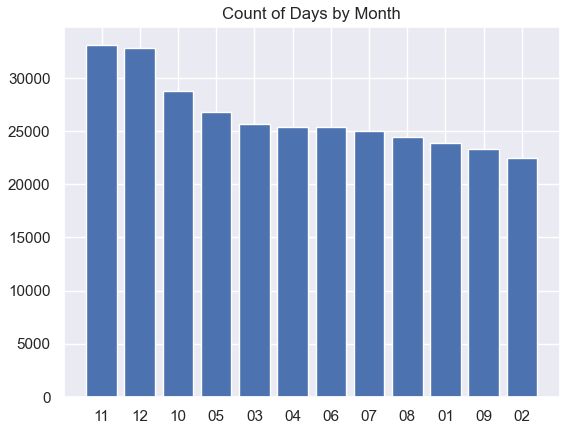
\includegraphics[height=0.40\textwidth]{conteo.png} % Ajusta el ancho de la imagen
    \label{fig:etiqueta_imagen} % Etiqueta para referirse a la imagen en el texto
\end{figure}

Furthermore, seasonal mean production of the obtained data can be observed in Figure 2.

\begin{figure}[H] % [H] coloca la imagen exactamente en el lugar donde aparece en el texto
    \centering % Centra la imagen
    \caption{Mean production by day and season of the year} % Leyenda de la imagen
    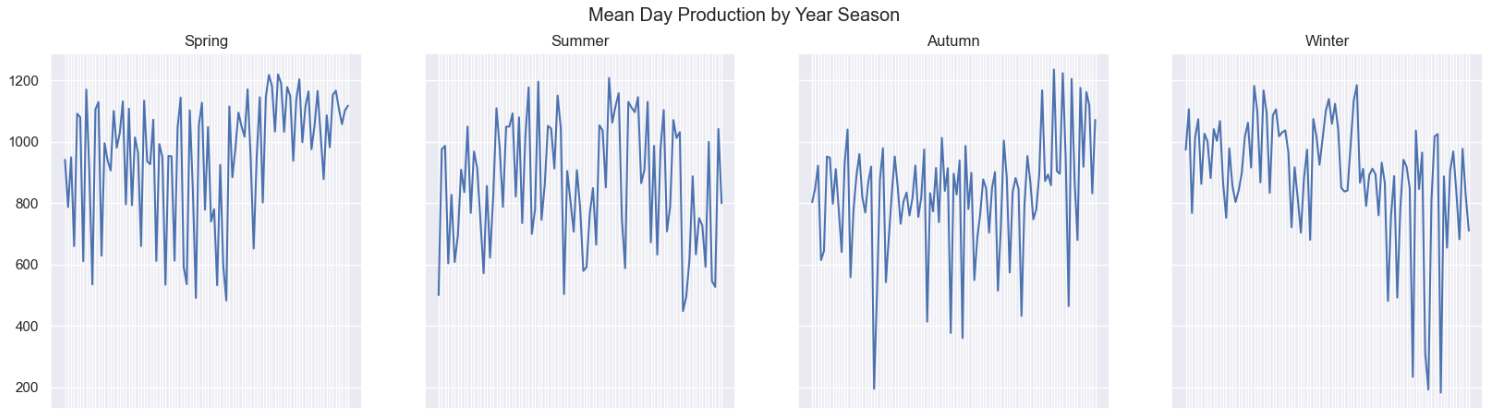
\includegraphics[width=1\textwidth]{temporada.png} % Ajusta el ancho de la imagen
    \label{fig:etiqueta_imagen} % Etiqueta para referirse a la imagen en el texto
\end{figure}

\section{Time Series Analysis}
As the data is ready to be used in models, this section takes on the performed time series analysis. First of all, the first ten days of the data can be seen on the following graph

\begin{figure}[H] % [H] coloca la imagen exactamente en el lugar donde aparece en el texto
    \centering % Centra la imagen
    \caption{First ten days of SPV generation} % Leyenda de la imagen
    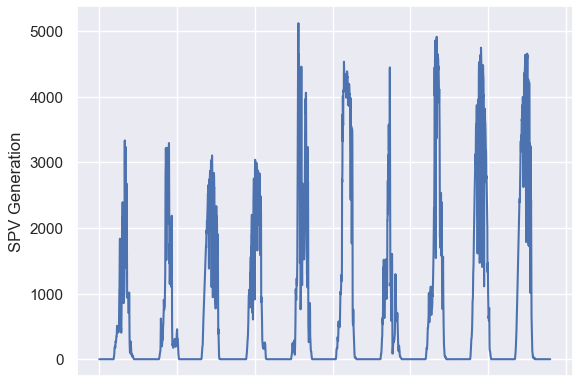
\includegraphics[height=0.35\textwidth]{tendays.png} % Ajusta el ancho de la imagen
    \label{fig:etiqueta_imagen} % Etiqueta para referirse a la imagen en el texto
\end{figure} 

Performing a augmented Dickey-Fuller test results can be seen in Table 4.

\begin{table}[H]
    \centering
    \caption{Descriptive statistics for some relevant columns}
    \begin{tabular}{>{\raggedright\arraybackslash}p{5cm} p{5cm}} % Ajusta el ancho de las columnas según sea necesario
        \toprule
        \textbf{Values} & \textbf{Metric} \\
        \midrule
        -57.682661 & Test Statistics \\
        0.000000 & p-value \\
        76.000000 & No. of lags used \\
        158927.000000 & Number of observations used \\
        -3.430391 & Critical value (1\%) \\
        -2.861558 & Critical value (5\%) \\
        -2.566780 & Critical value (10\%) \\
        \bottomrule
    \end{tabular}
    \caption{Dickey-Fuller test results}
\end{table}

From this values we can observe that the time series is stationary since the p-value is not greater than 5\%, this can also be observed in the time series decomposition in Figure 4.

\begin{figure}[H] % [H] coloca la imagen exactamente en el lugar donde aparece en el texto
    \centering % Centra la imagen
    \caption{Time series decomposition of the SPV generation time series} % Leyenda de la imagen
    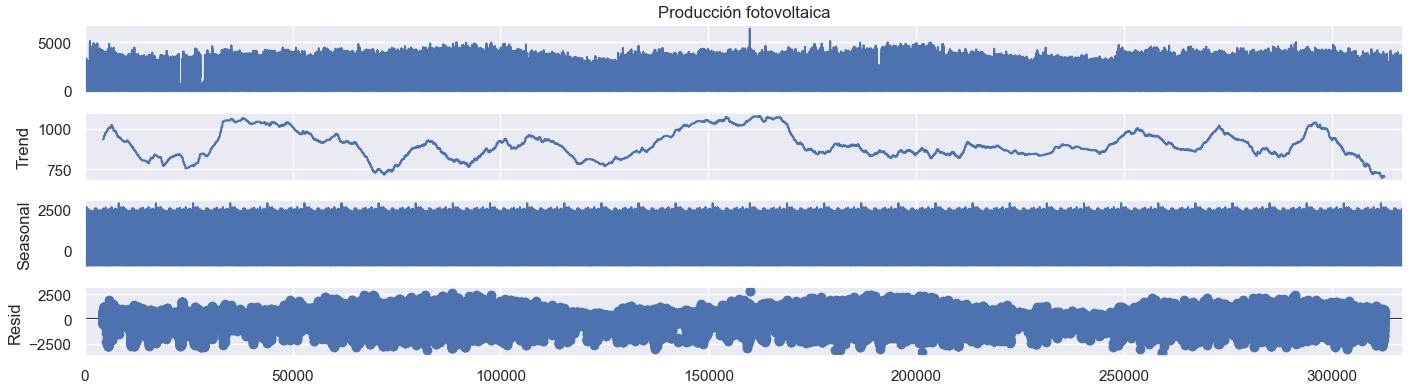
\includegraphics[width=1\textwidth]{decomposition.png} % Ajusta el ancho de la imagen
    \label{fig:etiqueta_imagen} % Etiqueta para referirse a la imagen en el texto
\end{figure} 

The trend does not increase or decrease.

\subsection{Time Series Forecasting}
The forecasting was realized following the next train/test split.

\begin{figure}[H] % [H] coloca la imagen exactamente en el lugar donde aparece en el texto
    \centering % Centra la imagen
    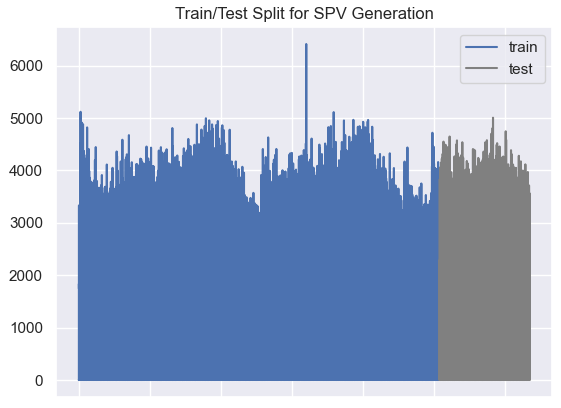
\includegraphics[height=0.35\textwidth]{traintest.png} % Ajusta el ancho de la imagen
    \caption{Time series decomposition of the SPV generation time series} % Leyenda de la imagen
    \label{fig:etiqueta_imagen} % Etiqueta para referirse a la imagen en el texto
\end{figure} 

After fitting the ARIMA model the following results can be observed.

\begin{figure}[H] % [H] coloca la imagen exactamente en el lugar donde aparece en el texto
    \centering % Centra la imagen
    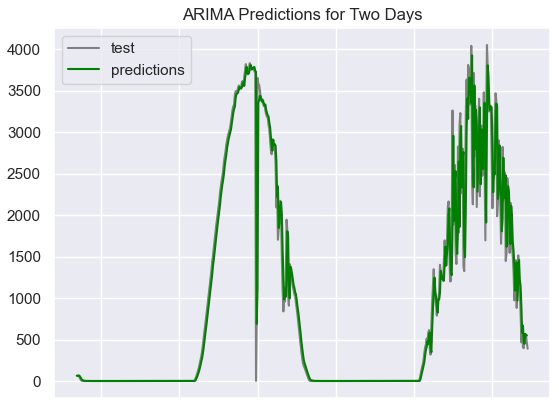
\includegraphics[height=0.35\textwidth]{ARIMA.png} % Ajusta el ancho de la imagen
    \caption{ARIMA Predictions of Two Days} % Leyenda de la imagen
    \label{fig:etiqueta_imagen} % Etiqueta para referirse a la imagen en el texto
\end{figure} 

The results of the time series forecasting model demonstrated a mean squared error (MSE) of 143,068.8. While this value indicates the model's ability to capture the underlying patterns of the data, it also suggests there is room for improvement in terms of accuracy. Factors such as model complexity, feature selection, and parameter tuning could be further optimized to reduce prediction error. Overall, the results confirm the model's potential but highlight the need for more refined approaches to achieve better forecasting performance.

\section{LSTM}
Training the LSTM model follows the train/test. The LSTM model is configured with RELU as activation function, the model was trained for 100 epochs and a batch size of 128. The results can be seen on the following graph

\begin{figure}[H] % [H] coloca la imagen exactamente en el lugar donde aparece en el texto
    \centering % Centra la imagen
    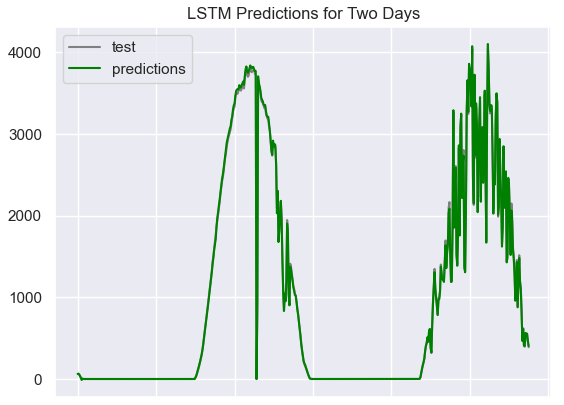
\includegraphics[height=0.35\textwidth]{LSTM.png} % Ajusta el ancho de la imagen
    \caption{LSTM Predictions of Two Days} % Leyenda de la imagen
    \label{fig:etiqueta_imagen} % Etiqueta para referirse a la imagen en el texto
\end{figure} 

The implementation of the Long Short-Term Memory (LSTM) model yielded a mean squared error (MSE) of 571.8, demonstrating a significant improvement in forecasting accuracy compared to traditional methods. This low error indicates that the LSTM effectively captured the temporal dependencies and complex patterns inherent in the data. The results underscore the strength of LSTM networks in handling sequential data, making them a powerful tool for time series forecasting. However, there remains an opportunity to enhance model performance further through techniques such as hyperparameter optimization, regularization, and incorporating additional features.

\section{Conclusion and Future Work}
This paper presented a comparative analysis of time series forecasting methods, highlighting the effectiveness of Long Short-Term Memory (LSTM) networks in capturing complex temporal patterns. The traditional time series forecasting model achieved a mean squared error (MSE) of 143,068.8, illustrating the inherent challenges in accurately predicting outcomes based on historical data. In contrast, the LSTM model demonstrated a substantial improvement with an MSE of 571.8, showcasing its capability to learn long-range dependencies and effectively handle sequential data.

These results underscore the advantages of using LSTM networks for time series forecasting, particularly in scenarios where data exhibits intricate patterns and correlations over time. While the LSTM model showed promising accuracy, there remains potential for further enhancement through hyperparameter tuning and the integration of additional features.

Future research should focus on refining these models and exploring hybrid approaches that combine the strengths of both traditional and advanced techniques. By continuing to improve forecasting accuracy, we can enhance decision-making processes across various applications, from finance to resource management.


\begin{thebibliography}{99}
\bibitem{referencia1}
Si J., Cai Y., Wang Y., Liu H., Song W., Liu Q., Su X., and Ren J. "Piecewise Clustering Prediction Model of Distributed Photovoltaic Power Based on Principal Component Analysis", 2021 IEEE IAS Industrial and Commercial Power System Asia, pp. 437-443, July 2021.

\bibitem{referencia2}
Sanz-Gorrachategui P., Pastor-Flores A., Guillén-Asensio J.S., Artal-Sevil A., Bono-Nuez
B., Martín-del-Brío C., and Bernal-Ruiz C. "Unsupervised clustering of battery waveforms in off grid PV installations", 2020 Fifteenth International Conference on Ecological Vehicles and Renewable Energies (EVER).

\bibitem{referencia3}
Pulipaka S. and Kumar R. "Power prediction of soiled PV module with neural networks using hybrid data clustering and division techniques", Solar Energy vol. 133 (2016), pp. 485-500

\bibitem{referencia4}
Munshi A. and Mohamed Y. "Photovoltaic power pattern clustering based on conventional and swarm clustering methods", Solar Energy vol. 124 (2016),pp.39-56

\bibitem{referencia5}
Feng C., Cui M., Hodge B., Lu S., Hamann H. and Zhang J. "Unsupervised Clustering-Based Short Term Solar Forecasting", IEEE Transactions on Sustainable Energy, vol. 10, no.4, October 2019

\bibitem{referencia6}
Chatfield, C. (2003). The Analysis of Time Series: An Introduction (6th ed.). Chapman \& Hall/CRC.

\bibitem{referencia7}
Box, G. E. P., Jenkins, G. M., Reinsel, G. C., \& Ljung, G. M. (2015). Time Series Analysis: Forecasting and Control (5th ed.). Wiley.

\bibitem{referencia8}
Goodfellow, I., Bengio, Y., \& Courville, A. (2016). Deep Learning. MIT Press.

\bibitem{referencia9}
Hochreiter, S., and Schmidhuber, J. "Long Short-Term Memory", Neural Computation, vol. 9, no. 8 (1997), pp. 1735-1780.

\end{thebibliography}

\end{document}
